\section{Installation and update}

\subsection{Installing}

\begin{frame}
\frametitle{Installing Python}

\begin{description}

\item<1->[Hard way:] download source and compile:\\
\url{https://www.python.org/downloads/}

\item<2->[Normal way:] use installer or package:

\begin{itemize}
\item Windows: \url{https://www.python.org/downloads/windows/}
\item Mac OS: \url{https://www.python.org/downloads/mac-osx/}
\item Linux: package manager:\\
python2.x and python2.x-dev packages
\end{itemize}

\item<3->[Easy way:] Python distributions such as:\\
\href{https://www.continuum.io/downloads}{Anaconda} \comment{free}\\
\href{https://www.enthought.com/products/canopy/}{Enthought Canopy} \comment{free and commercial}\\
\href{http://python-xy.github.io/}{Python(x,y)} \comment{free, Windows only}\\
+ others

\end{description}

\end{frame}

%--------------------------------------------------------------------------------------------------------------
\begin{frame}[fragile]
\frametitle{Installing modules}

Example: SciPy (\url{http://www.scipy.org/}):\\
mathematics, science, and engineering

\begin{description}
\item<2->[Easy way:] Windows, Linux, Mac:\\
use Scientific Python distribution
\item<3->[Intermediate:] Linux, Mac: install package\\
\begin{itemize}
\item Linux: package manager
\item Mac: MacPorts % used by Evan
\end{itemize}
\item<4->[Harder:] build from source
\begin{lstlisting}[language=bash]
 $ python setup.py install
\end{lstlisting}
\item<5->[Better:] pip
\end{description}

\end{frame}


%--------------------------------------------------------------------------------------------------------------
\begin{frame}[fragile]
\frametitle{Using \texttt{pip} to manage modules}

\texttt{pip} = recommended tool for installing Python packages

\begin{description}
\item<2->[Installation:]
\begin{itemize}
\item Included in recent Python version
\item Otherwise: download and run \pyfile{get-pip.py}\\
\url{https://pip.pypa.io/en/stable/installing/\#install-pip}
\begin{lstlisting}[language=bash]
$ python get-pip.py
\end{lstlisting}
\end{itemize}

\item<3->[Usage:]
\begin{itemize}
\item Install latest version + dependencies:
\begin{lstlisting}[language=bash]
$ pip install Package
\end{lstlisting}

\item Specify exact version:
\begin{lstlisting}[language=bash]
$ pip install Package==x.y.z
\end{lstlisting}
\item Specify minimum version:
\begin{lstlisting}[language=bash]
$ pip install 'Package>=x.y.z'
\end{lstlisting}
\end{itemize}

\end{description}

\end{frame}

%--------------------------------------------------------------------------------------------------------------
\begin{frame}[t, fragile]
\frametitle{More about \texttt{pip}}

\defverbatim{\piplist}{%
\tiny
\begin{verbatim}
aptoncd (0.1.98-bzr117-1.2)
backports.ssl-match-hostname (3.4.0.2)
basemap (1.0.7)
...
xhtml2pdf (0.0.6)
zope.interface (3.6.1)
\end{verbatim}
}

\defverbatim{\pipfreeze}{%
\tiny
\begin{verbatim}
aptoncd===0.1.98-bzr117-1.2
backports.ssl-match-hostname==3.4.0.2
basemap==1.0.7

...
xhtml2pdf==0.0.6
zope.interface==3.6.1
\end{verbatim}
}

\defverbatim{\pipshow}{%
\tiny
\begin{verbatim}
%---
%Metadata-Version: 1.1
%Name: numpy
%Version: 1.9.2
%Summary: NumPy: array processing for numbers, strings, records, and objects.
...
%Requires:
\end{verbatim}
}

\begin{itemize}
\item<1-> Uninstall packages:                   
\begin{lstlisting}[language=bash]
$ pip uninstall
\end{lstlisting}
\item<2->List installed packages:
\begin{lstlisting}[language=bash]
$ pip list
\end{lstlisting}
\onslide*<2>{\tiny \piplist}
\item<3-> Output installed packages in requirements format:
\begin{lstlisting}[language=bash]
$ pip freeze
\end{lstlisting}
\onslide*<3>{\pipfreeze}
\item<4-> Show information about installed packages:
\begin{lstlisting}[language=bash]
$ pip show Package
\end{lstlisting}
\onslide*<4>{\pipshow}
\end{itemize}

\end{frame}

%--------------------------------------------------------------------------------------------------------------
%\begin{frame}[fragile]
%\frametitle{Managing modules with Anaconda}
%
%http://conda.pydata.org/docs/using/pkgs.html
%
%
%\end{frame}

%--------------------------------------------------------------------------------------------------------------
\subsection{Running your code}
\begin{frame}[fragile, t]
\frametitle{Running your code: several solutions}

\begin{enumerate}
\item<1-> Edit, then run in a shell:
\begin{lstlisting}[language=bash]
$ python mycode.py
\end{lstlisting}
or 
\begin{lstlisting}[language=bash]
$ mycode.py
\end{lstlisting}

% Add ipython + magic functions + autocomplete etc


\item<2-> Use an \textit{Integrated Development Environment} (IDE)\\
(editor + build automation tools + debugger):\\
Atom, Eclipse, PyCharm, Idle, \ldots\\
Complete list: \url{https://wiki.python.org/moin/PythonEditors}
\item<3-> Write an \textit{ipython notebook}\\
(interactive computational environment):\\
\url{http://ipython.org/notebook.html} \comment{(see Programming in Python 2)}
\end{enumerate}

\end{frame}

%--------------------------------------------------------------------------------------------------------------
\begin{frame}[c]
\frametitle{What do we work with?}
\huge
\faLaptop~examples\ldots

\vfill 
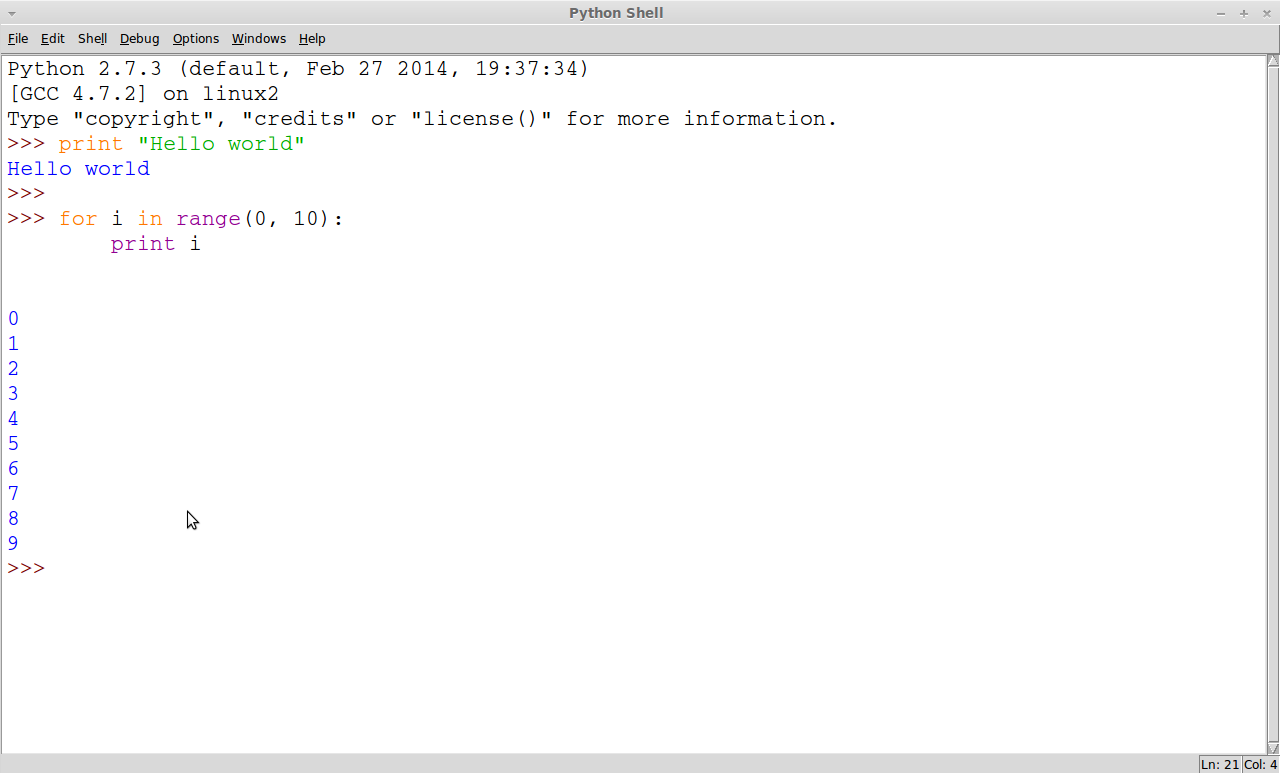
\includegraphics[width=.45\textwidth]{python_idle}~~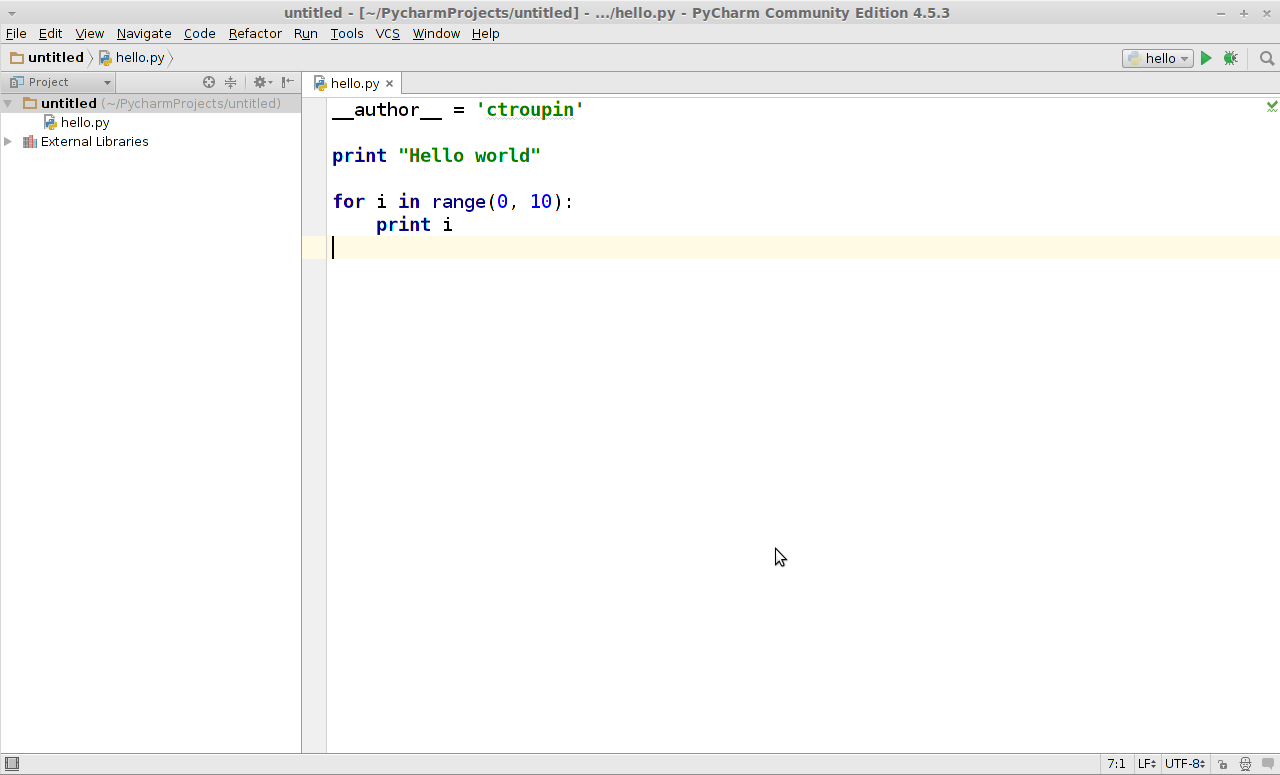
\includegraphics[width=.45\textwidth]{python_pycharm}

% Here we will say what we use personaly, type of workflow etc
\end{frame}
